\documentclass[../HWThesis.tex]{subfiles}
\begin{document}
\chapter{Background}
\label{ch:background}


This thesis comes set up with acronyms so you can define terms you use repeatedly and make sure they're formatted correctly every time. A simple acronym is  \ac{lol}.

Now it is defined, we henceforth just print \ac{lol}.


\section{Section}
Of course acronyms are perhaps best used for longer terms like species, proteins, part names, or very specific phrases, for example the phrase: \\ \ac{woodchuck}

Which is now conveniently shortened to \ac{woodchuck}

\begin{figure}[H]
 \begin{center}
 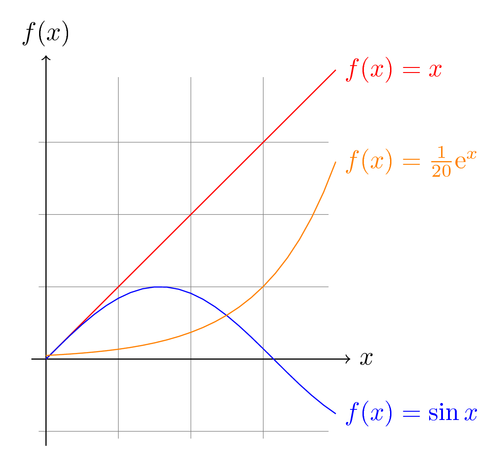
\includegraphics [width=12cm]{Background/pic.png}
 \caption{Figure Caption.}
 \label{fig:label}
\end{center}
\end{figure} 

\cite{gum, ghc-smp}

\subsection{Subsection}

\begin{table}[H]
\begin{center}
\begin{tabular}{c c c c} % centered columns (4 columns)
\hline\hline %inserts double horizontal lines
Case & Method\#1 & Method\#2 & Method\#3 \\ [0.5ex] % inserts table 
%heading
\hline % inserts single horizontal line
1 & 50 & 837 & 970 \\ % inserting body of the table
2 & 47 & 877 & 230 \\
3 & 31 & 25 & 415 \\
4 & 35 & 144 & 2356 \\
5 & 45 & 300 & 556 \\ [1ex] % [1ex] adds vertical space
\hline %inserts single line
\end{tabular}\caption{Table Caption}
\label{tab:lable}
\end{center}
\end{table}


\subsubsection{Subsubsection}

\end{document}
